\chapter{From Discrete to Continuous}

\begin{goals}
\begin{itemize}
    \item Understand why we need to ``soften'' discrete structures
    \item See concrete examples: soft attention, soft selection
    \item Introduce the idea of relaxation and rounding
\end{itemize}
\end{goals}

\section{The Continuization Trick}

Discrete optimization is hard. Continuous optimization has gradients.

\textbf{Strategy}:
\begin{enumerate}
    \item Embed discrete objects into a continuous space
    \item Optimize in the continuous space
    \item Round back to discrete
\end{enumerate}

\section{Example: Soft Selection}

\textbf{Discrete}: Choose one of $n$ items. Represented as one-hot vector $e_i \in \{0,1\}^n$.

\textbf{Continuous}: Use a probability distribution $p \in \Delta^{n-1}$ (the simplex).

\begin{center}
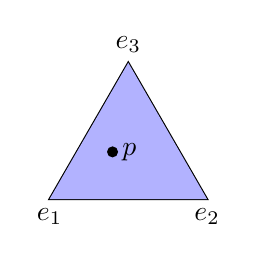
\begin{tikzpicture}[scale=2]
% Simplex
\draw[thick] (0,0) -- (1,0) -- (0.5, 0.866) -- cycle;
\node[below] at (0,0) {$e_1$};
\node[below] at (1,0) {$e_2$};
\node[above] at (0.5, 0.866) {$e_3$};
\fill[blue!30] (0,0) -- (1,0) -- (0.5, 0.866) -- cycle;
\fill (0.4, 0.3) circle (1pt) node[right] {$p$};
\end{tikzpicture}
\end{center}

The corners are discrete choices. The interior is ``soft'' mixtures.

\section{Example: Soft Transitions}

\textbf{Discrete}: Transition relation $R \subseteq W \times W$. Either $(w, v) \in R$ or not.

\textbf{Continuous}: Transition weights $R : W \times W \to [0, 1]$.

\begin{itemize}
    \item $R(w, v) = 1$: definitely connected
    \item $R(w, v) = 0$: definitely not connected
    \item $R(w, v) = 0.7$: ``70\% connected'' (soft)
\end{itemize}

\section{The Softmax Function}

To go from unconstrained $\mathbb{R}^n$ to the simplex:
\[
\mathrm{softmax}(z)_i = \frac{e^{z_i}}{\sum_j e^{z_j}}
\]

\begin{itemize}
    \item Output is always a valid distribution
    \item Differentiable everywhere
    \item Temperature $\tau$: $\mathrm{softmax}(z/\tau)$ becomes sharper as $\tau \to 0$
\end{itemize}

\section{Relaxation and Rounding}

\textbf{Relaxation}: Replace discrete constraints with continuous ones.
\[
x \in \{0, 1\} \quad \rightsquigarrow \quad x \in [0, 1]
\]

\textbf{Rounding}: After optimization, snap back to discrete.
\[
x = 0.7 \quad \rightsquigarrow \quad x = 1
\]

\begin{warning}
Rounding can fail! The continuous optimum might round to a bad discrete solution. This is why we need careful design of the relaxation.
\end{warning}

\section{What We Need}

To make this systematic, we need:
\begin{enumerate}
    \item A principled way to ``soften'' logical operations ($\land, \lor, \neg$)
    \item Compatibility with gradient computation
    \item Convergence guarantees (soft $\to$ crisp)
\end{enumerate}

This is exactly what \textbf{semirings} provide.
